\documentclass[11pt]{article}
\usepackage{geometry, titlesec}
\usepackage[parfill]{parskip}
\usepackage[italicdiff]{physics}
\usepackage{amsfonts, amsthm}
\usepackage[cm]{fullpage}
\usepackage{fancyhdr}
\usepackage{enumitem}
\usepackage{xcolor, soul}
\usepackage{graphicx}
\usepackage[export]{adjustbox}
\usepackage{siunitx}
\usepackage{hyperref}
%\allowdisplaybreaks

\renewcommand{\thesubsection}{\thesection.\alph{subsection}}
\setenumerate[1]{label={(\alph*)}}

\makeatletter
\renewcommand*\env@cases[1][1.2]{%
  \let\@ifnextchar\new@ifnextchar
  \left\lbrace
  \def\arraystretch{#1}%
  \array{@{}l@{\quad}l@{}}%
}
\makeatother
 
\renewcommand{\footrulewidth}{.2pt}
%\setlist[enumerate]{leftmargin=*}
\pagestyle{fancy}
\fancyhf{}
\lhead{Physics 132-B}
\chead{\textbf{Discussion 4 Solutions}}
\rhead{A--De Discussion}
\setlength{\headheight}{11pt}
\setlength{\headsep}{11pt}
\setlength{\footskip}{24pt}
\lfoot{\today}
\rfoot{\thepage}

\titleformat{\subsection}[runin]{\normalfont\large\bfseries}{\thesubsection}{1em}{}
\newcommand{\refeq}[1]{(\ref{#1})}

\newcommand{\beq}{\begin{equation*}}
\newcommand{\eeq}{\end{equation*}}

\newcommand{\beqn}{\begin{equation}}
\newcommand{\eeqn}{\end{equation}}

\newcommand{\blg}{\begin{align*}}
\newcommand{\elg}{\end{align*}}


\newenvironment{statement}
{
%    \color{gray}
    \ignorespaces
}
{
%    \smallskip
}

\newenvironment{problem}
{
    \color{darkgray}
    \ignorespaces
}

\newenvironment{solution}
{
    \paragraph{Solution}
    \ignorespaces
}
{
    \bigskip
}

\renewcommand{\vec}[1]{\mathbf{#1}}


\begin{document}
	

\newcommand{\vE}{\vec{E}}
\newcommand{\vEq}{\vE_1}
\newcommand{\vEw}{\vE_2}
\renewcommand{\qq}{q_1}
\newcommand{\qw}{q_2}
\newcommand{\tht}{\theta}
\newcommand{\thtq}{\tht_1}
\newcommand{\thtw}{\tht_2}
\newcommand{\Eq}{E_1}
\newcommand{\Ew}{E_2}
\newcommand{\Ex}{E_x}
\newcommand{\Ey}{E_y}
\newcommand{\ent}{\epsilon_0}
\newcommand{\fk}{\frac{1}{4\pi\ent}}

\begin{minipage}[l]{0.65\textwidth}
\paragraph{Problem 21.96}
%\paragraph{Problem 1}
\begin{problem}
	Two charges are placed as shown in Fig.~P21.96.  The magnitude of $\qq$ is \SI{3.00}{\micro\coulomb}, but its sign and the value of the charge $\qw$ are not known.  The direction of the net electric field $\vE$ at point $P$ is entirely in the negative $y$ direction. \medskip
	\begin{enumerate}
		\item Considering the different possible signs of $\qq$ and $\qw$, four possible diagrams could represent the electric fields $\vEq$ and $\vEw$ produced by $\qq$ and $\qw$.  Sketch the four possible electric field configurations. \medskip
		\item Using the sketches from part (a) and the direction of $\vE$, deduce the signs of $\qq$ and $\qw$. \medskip
		\item Determine the magnitude of $\vE$.
	\end{enumerate}
\end{problem}
\end{minipage}%
\hspace{0.05\textwidth}%
\begin{minipage}[r]{0.3\textwidth}
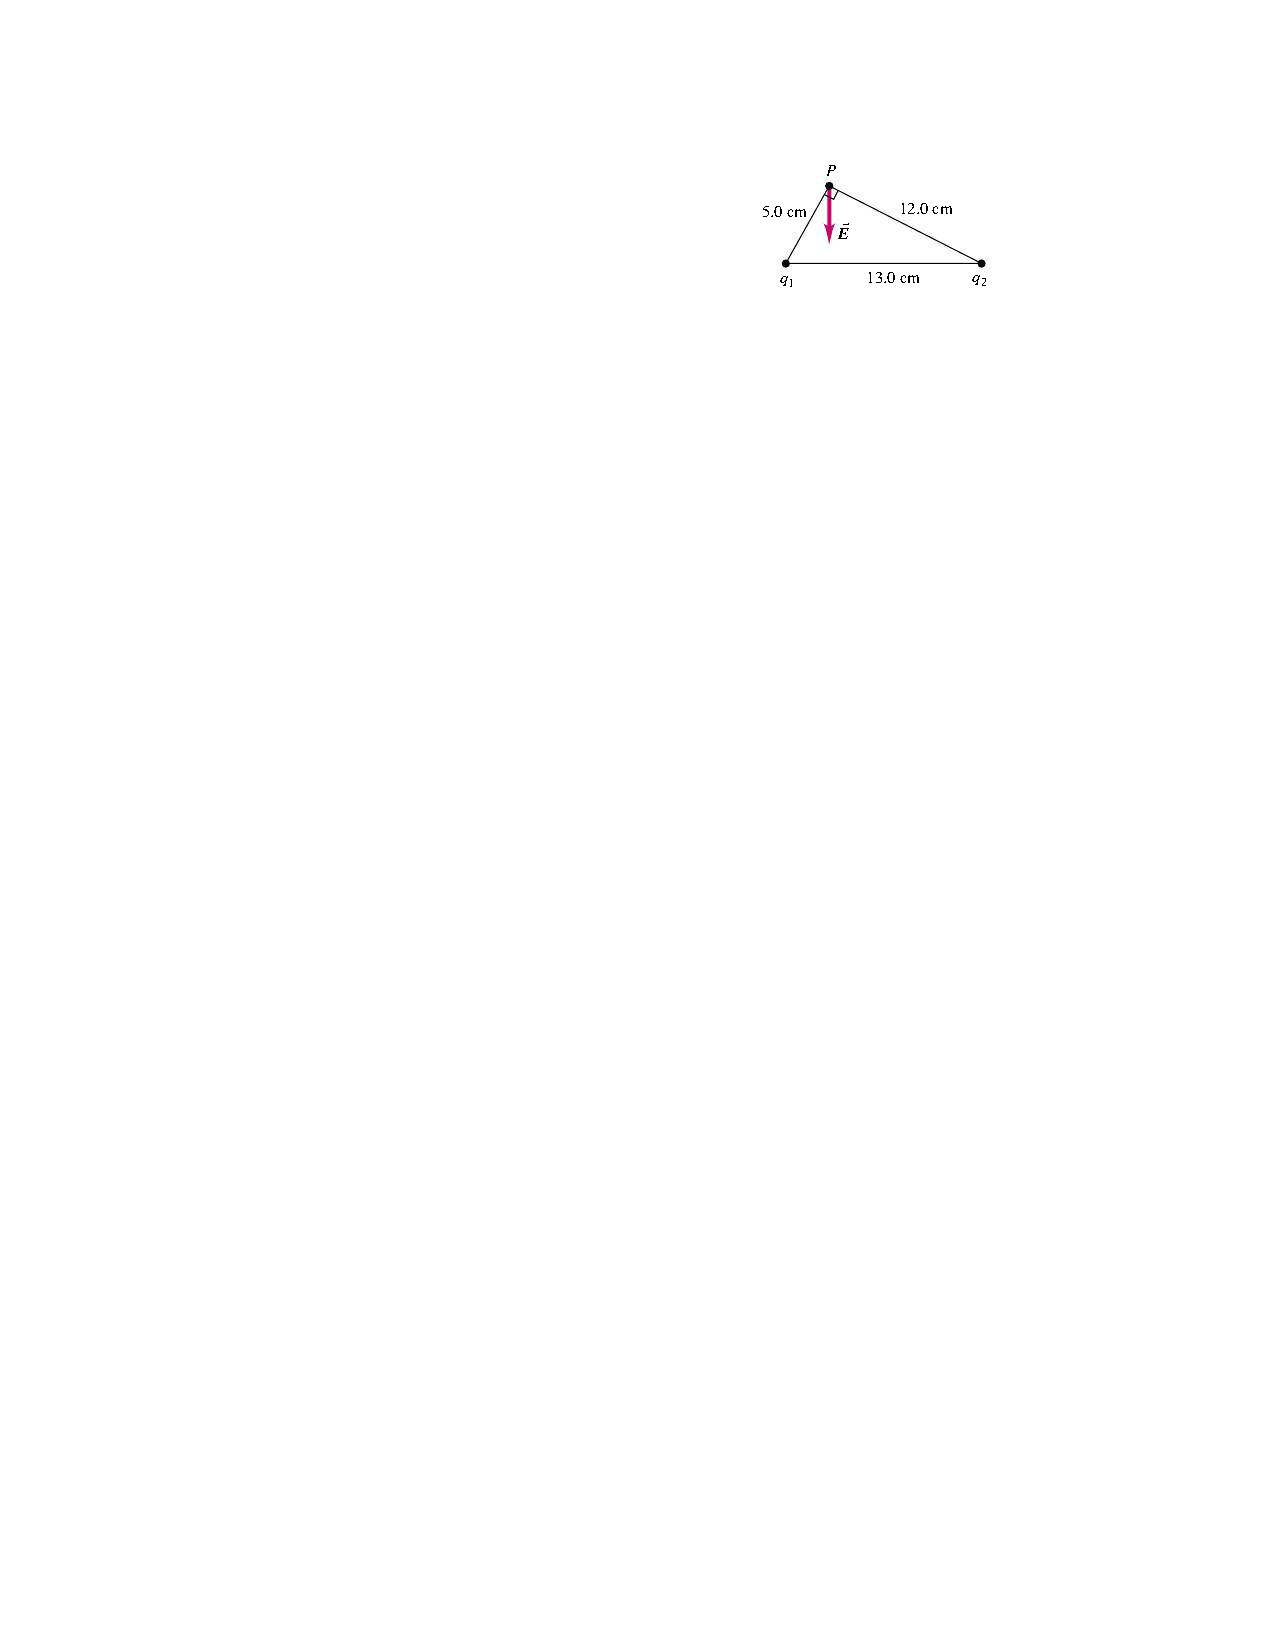
\includegraphics[width=\textwidth]{P21-96}
\center \textbf{Figure P21.96}
\end{minipage}

\begin{solution}
	\begin{enumerate}
		\item The four possible diagrams are:
		
		\begin{center}
			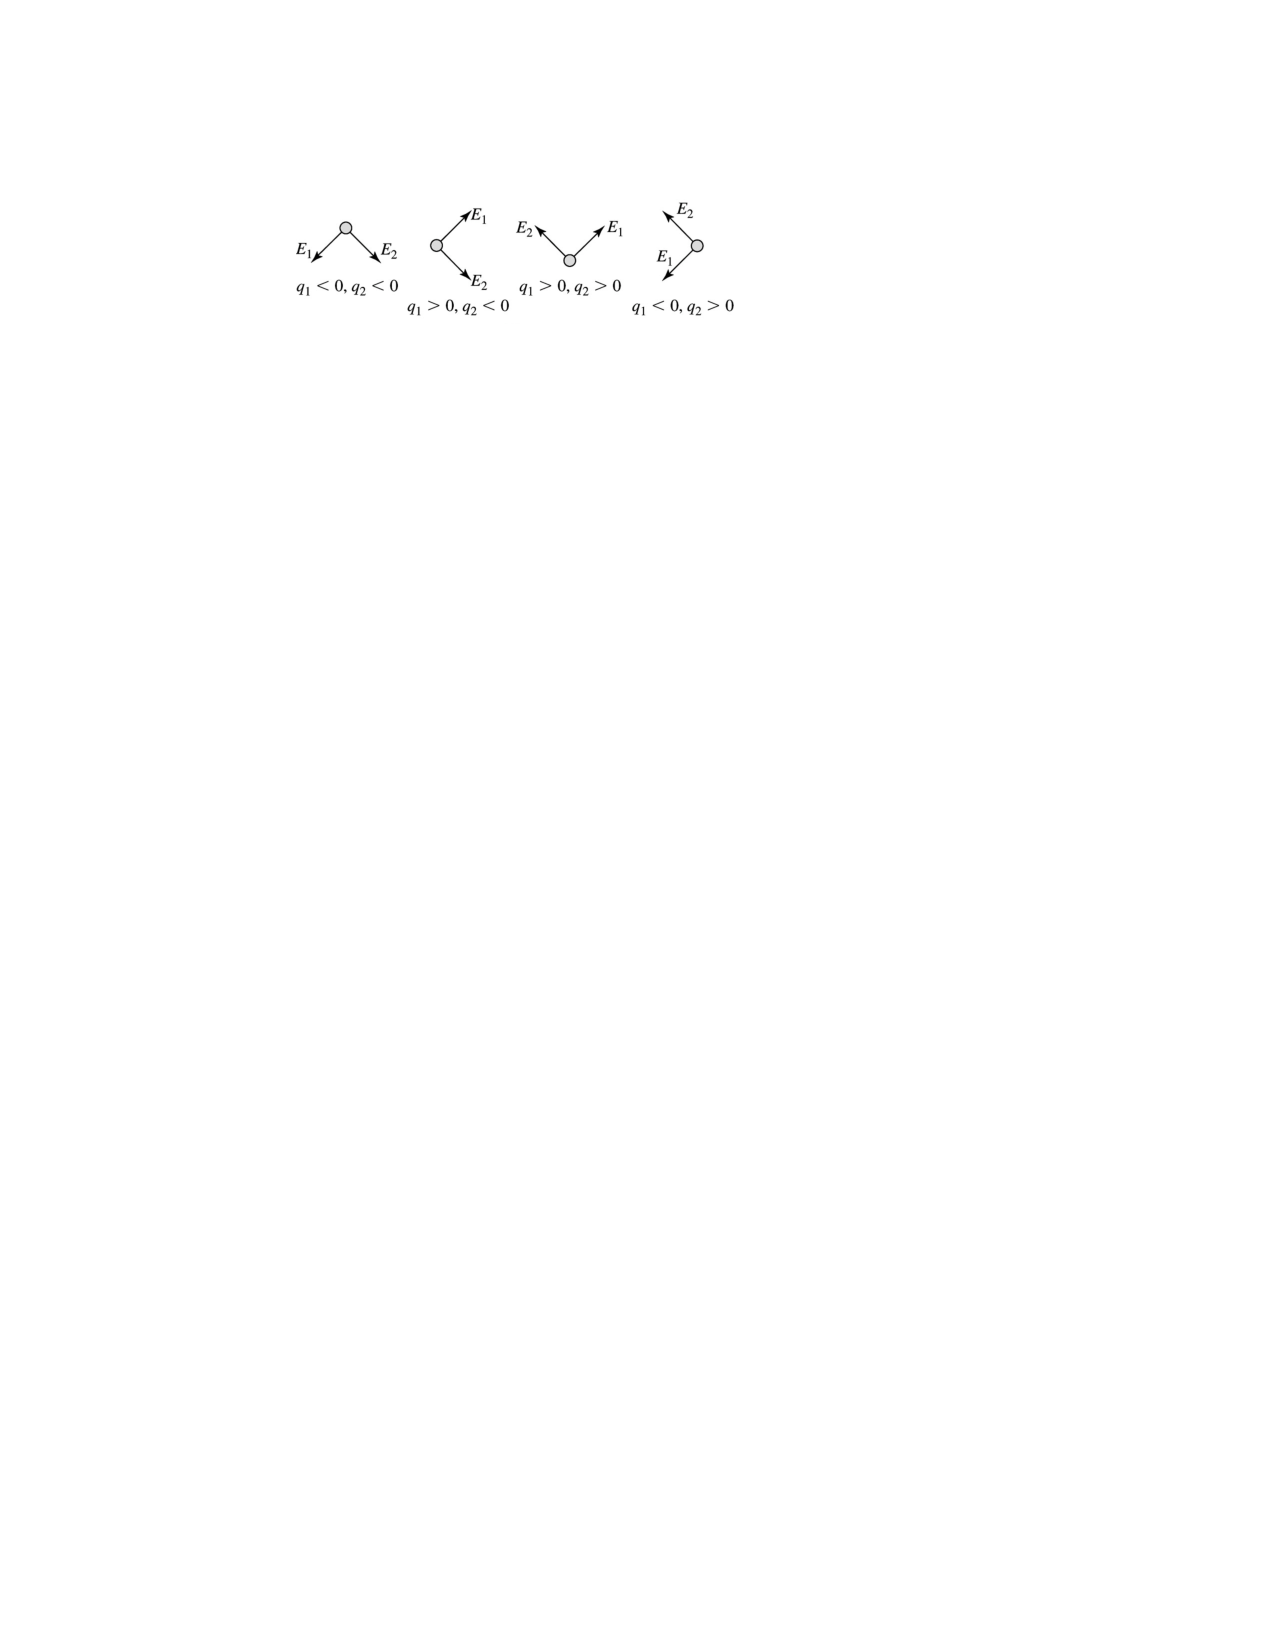
\includegraphics[scale=1.5]{P21-96a}
		\end{center}
		
		Here $E_1$ and $E_2$ indicate the electric fields of $\qq$ and $\qw$, respectively.
		
		\item The first diagram is the only one that has the net electric field $\vE = \vEq + \vEw$ pointing in the $-y$ direction like we want.  This means {\color{blue} both $\qq$ and $\qw$ are negative}.  (We also could have deduced this by placing a positive test charge at $P$, and realizing we need both $\qq$ and $\qw$ to be negative in order to produce an electric field pointing down.)
		
		\item Using the expression for the electric field due to a point charge, we can find the magnitudes of $\Eq$ and $\Ew$:
		\begin{align*}
			\Eq &= \fk \frac{\abs{\qq}}{(\SI{5.0}{\cm})^2} = -\fk \frac{\SI{3.00}{\micro\coulomb}}{(\SI{5.0}{\cm})^2}, &
			\Ew &= \fk \frac{\abs{\qw}}{(\SI{12.0}{\cm})^2}.
		\end{align*}
		Notice that we need to solve for $\qw$, which we can do by force balance.
		
		To find the magnitude of $\vE$, we need to find and add the $x$ and $y$ components of $\vEq$ and $\vEw$, which we can do by finding their angles from the horizontal.  Call these angles $\thtq$ and $\thtw$.  Building off of our diagram for (a), we can make something similar to a force diagram, but for the electric field:
		
		\begin{center}
			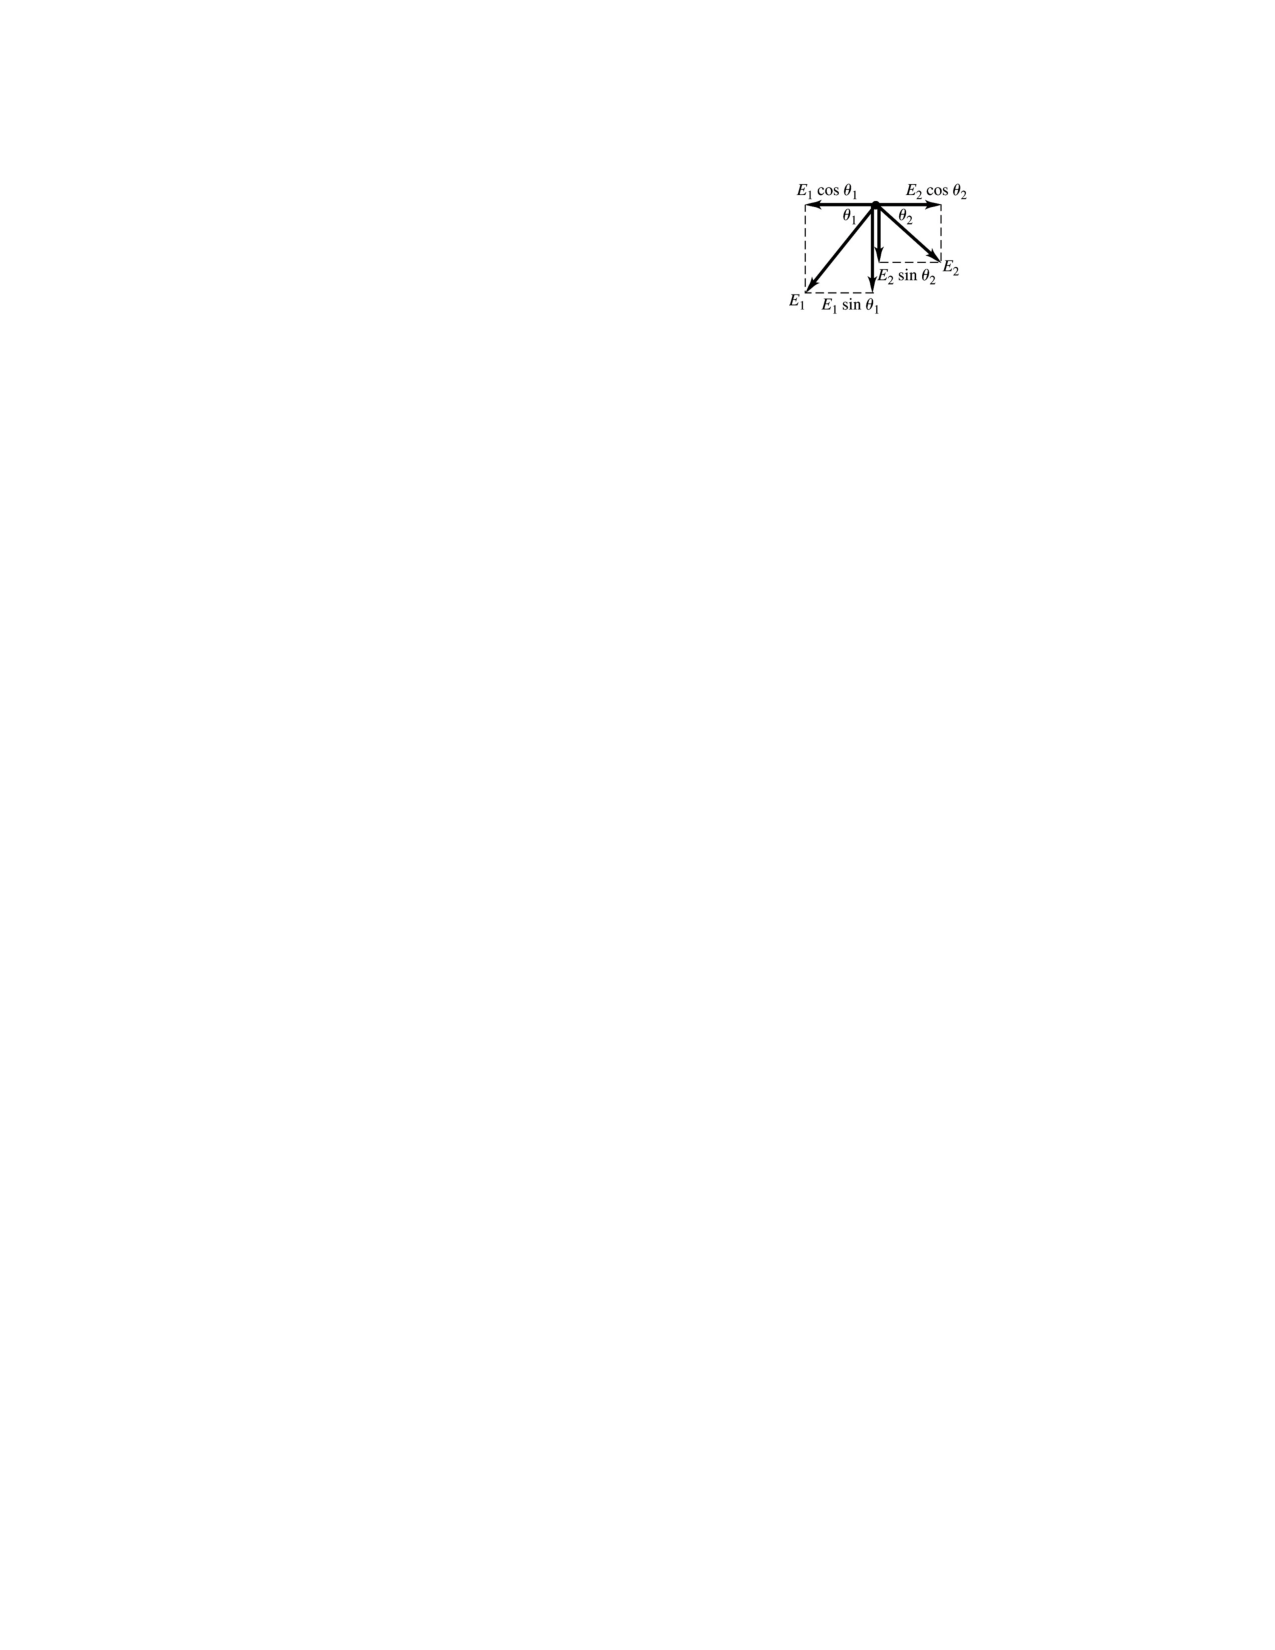
\includegraphics[scale=1.5]{P21-96b}
		\end{center}
		
		From Fig.~P21.96, we can write down
		\begin{align*}
			\cos\thtq &= \frac{5}{13}, &
			\sin\thtq &= \frac{12}{13}, &
			\cos\thtw &= \frac{12}{13}, &
			\sin\thtw &= \frac{5}{12}.
		\end{align*}
		
		First, let's balance forces in the $x$ direction, in which we know there's 0 net electric field.  This will allow us to find the magnitude of $\qw$:
		\beq
			0 = \Ex
			= {\Eq}_x + {\Ew}_x
			= \Eq \cos\thtq + \Ew \cos\thtw
			= -\frac{5}{13} \fk \frac{\SI{3.00}{\micro\coulomb}}{(\SI{5.0}{\cm})^2} + \frac{12}{13} \fk \frac{\abs{\qw}}{(\SI{12.0}{\cm})^2}
		\eeq
		\beq
			\implies \frac{\SI{3.00}{\micro\coulomb}}{\SI{5.0}{\square\cm}} = \frac{\abs{\qw}}{\SI{12.0}{\square\cm}}
			\implies \abs{\qw} = \frac{36}{5} \si{\micro\coulomb} = \SI{7.2}{\micro\coulomb}.
		\eeq
		
		Now we can add the forces in the $y$ direction to find the magnitude of $\vE$:
		\begin{align*}
			|\vE| &= \Ey
			= {\Eq}_y + {\Ew}_y
			= \Eq \sin\thtq + \Ew \sin\thtw
			= \frac{12}{13} \fk \frac{\SI{3.00}{\micro\coulomb}}{(\SI{5.0}{\cm})^2} + \frac{5}{12} \fk \frac{\SI{7.2}{\micro\coulomb}}{(\SI{12.0}{\cm})^2} \\
			&= \fk \left( \frac{12}{13} \frac{\SI{3.00e-6}{\coulomb}}{\SI{25e-4}{\square\m}} + \frac{5}{12} \frac{\SI{7.2e-6}{\coulomb}}{\SI{144e-4}{\square\m}} \right)
			= \fk \left( \frac{36}{325} + \frac{36}{1728} \right) \times\SI{e-2}{\coulomb\per\square\meter} \\
			&= (\SI{8.99e9}{\newton\square\meter\per\square\coulomb}) (\SI{0.131e-2}{\coulomb\per\square\meter}) \\
			&= {\color{blue} \SI{1.18e7}{\newton\per\coulomb}.}
		\end{align*}
	\end{enumerate}
\end{solution}

%\vfill

\newcommand{\dQ}{\dd{Q}}
\newcommand{\dz}{\dd{z}}
\newcommand{\du}{\dd{u}}
\newcommand{\dtht}{\dd{\tht}}
\newcommand{\ih}{\vec{\hat{i}}}

\paragraph{Problem 23.82}
%\paragraph{Problem 2}
\begin{problem}
	A hollow, thin-walled insulating cylinder of radius $R$ and length $L$ (like the cardboard tube in a roll of toilet paper) has charge $Q$ uniformly distributed over its surface.
	
	\begin{enumerate}
		\item Calculate the electric potential at all points along the axis of the tube.  Take the origin to be at the center of the tube, and take the potential to be zero at infinity.
		\setcounter{enumi}{2}
		\item Use the result of part (a) to find the electric field at all points along the axis of the tube.
	\end{enumerate}
\end{problem}

\begin{solution}
	\begin{enumerate}
		\item We can think of the tube as being made of a stack of charged rings, and integrate over the length of the stack.  Example~23.11 in the textbook derives the expression for the electric potential due to a ring, which is
		\beq
			V_\text{ring} = \fk \frac{Q_\text{ring}}{\sqrt{x^2 + a^2}},
		\eeq
		where $Q_\text{ring}$ is the total charge of the ring, $x$ is the distance from the center of the ring along its axis, and $a$ is the ring's radius~(Fig.~23.20).
			
		\begin{center}
			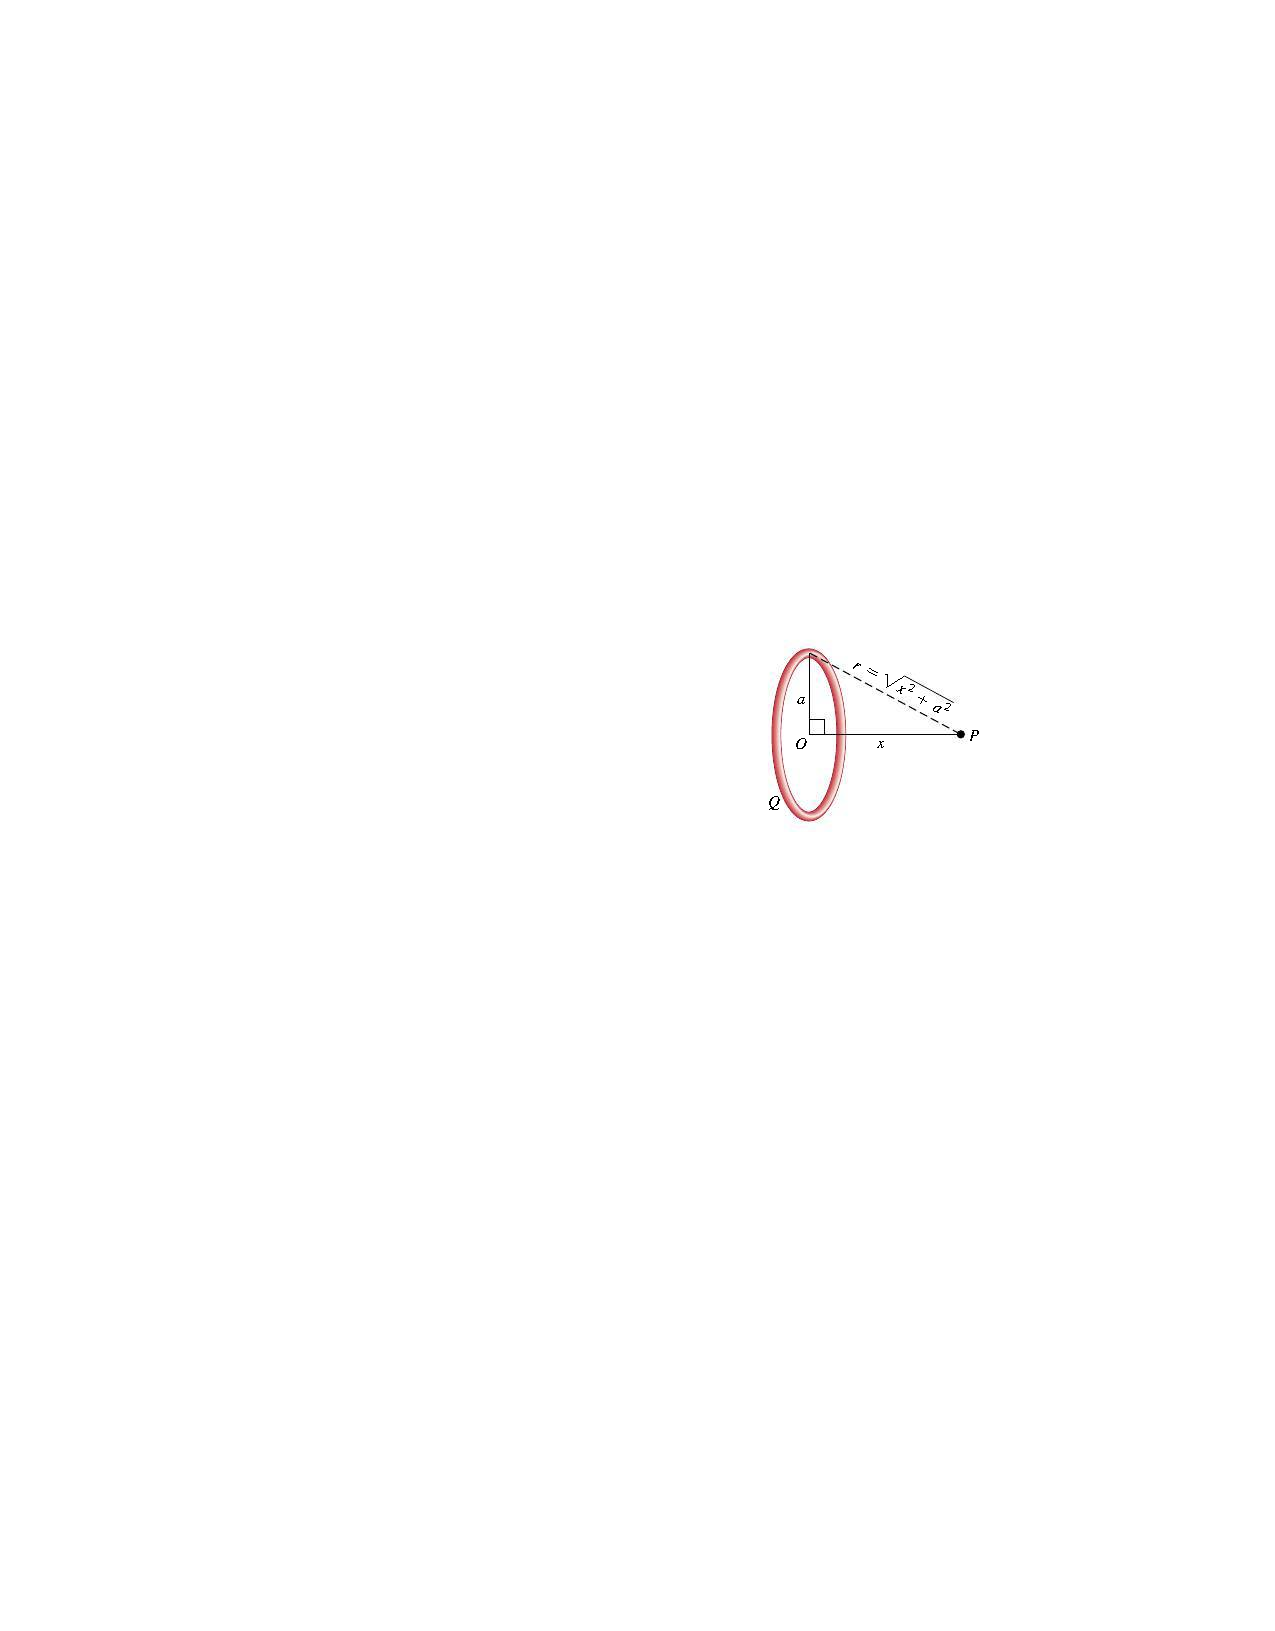
\includegraphics{23-20} \\
			\textbf{Figure 23.20}
		\end{center}

		Let the ring have charge $\dQ$ and be at position $z$ along the $x$ axis.  We will need to integrate $z$ from $-L/2$ to $L/2$.  The infinitesimal charge $\dQ$ of the ring is related to the entire charge of the tube through their respective lengths:
		\beq
			\frac{\dQ}{\dz} = \frac{Q}{L} \implies \dQ = \frac{Q}{L} \dz.
		\eeq
		Our integral is then
		\beq
			V = \int \fk \frac{\dQ}{\sqrt{(x-z)^2 + R^2}}
			= \fk \frac{Q}{L} \int_{-L/2}^{L/2} \frac{\dz}{\sqrt{(x-z)^2 + R^2}}.
		\eeq
		The denominator of the integrand looks kind of gross, so we probably want to do a $u$ substitution.  Let $u = x - z$, so $\du = -\dz$.  Then our integral becomes
		\beq
			V = -\fk \frac{Q}{L} \int_{x + L/2}^{x - L/2} \frac{\du}{\sqrt{u^2 + R^2}}
			= \fk \frac{Q}{L} \int_{x - L/2}^{x + L/2} \frac{\du}{\sqrt{u^2 + R^2}},
		\eeq
		whose form suggests a trig substitution.  Let $u = R \tan\tht$, so $\du = R \sec^2\tht \dtht$.  The the bounds of integration are
		\begin{align*}
			\thtq &\equiv \tan[-1](\frac{x - L/2}{R}), &
			\thtw &\equiv \tan[-1](\frac{x + L/2}{R}),
		\end{align*}
		and our integral becomes
		\begin{align*}
			V &= \fk \frac{Q}{L} \int_{\thtq}^{\thtw} \frac{R \sec^2\tht}{\sqrt{R^2 \tan^2\tht + R^2}} \dtht
			= \fk \frac{Q}{L} \int_{\thtq}^{\thtw} \frac{\sec^2\tht}{\sqrt{\tan^2\tht + 1}} \dtht
			= \fk \frac{Q}{L} \int_{\thtq}^{\thtw} \frac{\sec^2\tht}{\sqrt{\sec^2\tht}} \dtht \\
			&= \fk \frac{Q}{L} \int_{\thtq}^{\thtw} \sec\tht \dtht.
		\end{align*}
		This looks simple, but it's actually quite tricky to integrate.\footnote{In fact, it's so famously difficult there's even a \href{https://en.wikipedia.org/wiki/Integral_of_the_secant_function}{Wikipedia article} about it!}  It's not obvious what substitution we should use, since differentiating the cosine will give us a sine factor that won't cancel.  So it's best to consult a table of integrals for this one, which tells us
		\beq
			\int \sec\tht = \ln(\sec\tht + \tan\tht).
		\eeq
		Now we can plug in our bounds of integration:
		\begin{align*}
			V &= \fk \frac{Q}{L} \bigg[ \ln(\sec\tht + \tan\tht) \bigg]_{\thtq}^{\thtw}
			= \fk \frac{Q}{L} [ \ln(\sec\thtw + \tan\thtw) - \ln(\sec\thtq - \tan\thtq)] \\
			&= \fk \frac{Q}{L} \ln(\frac{\sec\thtw + \tan\thtw}{\sec\thtq + \tan\thtq})
			= \fk \frac{Q}{L} \ln(\frac{\sec(\tan[-1](\dfrac{x + L/2}{R})) + \tan(\tan[-1](\dfrac{x + L/2}{R}))}{\sec(\tan[-1](\dfrac{x - L/2}{R})) + \tan(\tan[-1](\dfrac{x - L/2}{R}))}) \\
			&= \fk \frac{Q}{L} \ln(\frac{\sqrt{1 + \left( \dfrac{x + L/2}{R} \right)^2} + \dfrac{x + L/2}{R}}{\sqrt{1 + \left( \dfrac{x - L/2}{R} \right)^2} + \dfrac{x - L/2}{R}})
			= {\color{blue} \fk \frac{Q}{L} \ln(\frac{\sqrt{R^2 + (x + L/2)^2} + x + L/2}{\sqrt{R^2 + (x - L/2)^2} + x - L/2})}.
		\end{align*}
		This is a really difficult problem.  No wonder we couldn't figure it out during the discussion period!
		
		
		\setcounter{enumi}{2}
		
		\newcommand{\Aq}{A_1}
		\newcommand{\Aw}{A_2}
		\newcommand{\Bq}{B_1}
		\newcommand{\Bw}{B_2}

		\clearpage
		\item Since the expression we found for $V$ depends only on $x$, we have
		\beq
			\vE = -\dv{V}{x} \,\ih,
		\eeq
		so we ``just'' have to differentiate with respect to $x$.  Judging by the expression we found for $V$, this will involve a lot of nasty algebra.  It's probably easier to integrate the expression for the electric field due to a ring over the length of the tube, like we did for the potential in (a).  We already did most of the substitution work.  Plus, the expression for the field has a different power of $x^2 + a^2$ in the denominator than the expression for the potential, so we won't even have to use a table of integrals.

		The electric field due to a ring of charge was found in Ex.~21.9 (and also in class):
		\beq
			E_\text{ring} = \fk \frac{Q_\text{ring} \, x}{(x^2 + a^2)^{3/2}}.
		\eeq
		Setting up the integral over the length of the tube as we did before, we get
		\beq
			E = \int \fk \frac{x}{[(x-z)^2 + R^2]^{3/2}} \dQ
			= \fk \frac{Q x}{L} \int_{-L/2}^{L/2} \frac{\dz}{[(x-z)^2 + R^2]^{3/2}}.
		\eeq
		Making the first substitution $u = x - z$,
		\beq
			E = \fk \frac{Q x}{L} \int_{x - L/2}^{x + L/2} \frac{\du}{(u^2 + R^2)^{3/2}},
		\eeq
		and then the second substitution $u = R \tan\tht$,
		\begin{align*}
			E &= \fk \frac{Q x}{L} \int_{\thtq}^{\thtw} \frac{R \sec^2\tht}{(R \tan^2\tht + R^2)^{3/2}} \dtht
			= \fk \frac{Q x}{L} \int_{\thtq}^{\thtw} \frac{\sec^2\tht}{(\sec^2\tht)^{3/2}} \dtht
			= \fk \frac{Q x}{L} \int_{\thtq}^{\thtw} \frac{\dtht}{\sec\tht} \\
			&= \fk \frac{Q x}{L} \int_{\thtq}^{\thtw} \cos\tht \dtht
			= \fk \frac{Q x}{L} \bigg[ \sin\tht \bigg]_{\thtq}^{\thtw}
			= \fk \frac{Q x}{L} (\sin\thtw - \sin\thtq).
		\end{align*}
		Much easier, right?  Now we just need to substitute back to our original variables:
		\begin{align*}
			\vE &= \fk \frac{Q x}{L} \left\{ \sin\!\left[ \tan[-1](\frac{x + L/2}{R}) \right] - \sin\!\left[ \tan[-1](\frac{x - L/2}{R}) \right] \right\} \ih \\
			&= \fk \frac{Q x}{L} \left( \frac{(x + L/2)/R}{\sqrt{(x + L/2)^2/R^2 + 1}} - \frac{(x - L/2)/R}{\sqrt{(x - L/2)^2/R^2 + 1}} \right) \ih \\
			&= {\color{blue} \fk \frac{Q x}{L} \left( \frac{x + L/2}{\sqrt{(x + L/2)^2 + R^2}} - \frac{x - L/2}{\sqrt{(x - L/2)^2 + R^2}} \right) \ih}.
		\end{align*}
		I promise Prof.~Gazes will never assign you a problem with calculus this difficult!
	\end{enumerate}
\end{solution}

%\bigskip \bigskip
\clearpage

\begin{minipage}[b]{0.65\textwidth}
\paragraph{Problem 22.32}
%\paragraph{Problem 3}
\begin{problem}
	A cube has sides of length $L = \SI{0.300}{\meter}$.  One corner is at the origin~(Fig.~E22.6).  The nonuniform electric field is given by ${\vE = (\SI{-5.00}{\newton\per\coulomb\per\meter}) x \, \ih + (\SI{3.00}{\newton\per\coulomb\per\meter}) z \, \vec{\hat{k}}}$. \medskip
	\begin{enumerate}
		\item Find the electric flux through each of the six cube faces $S_1,\ S_2,\ S_3,\ S_4,\ S_5$, and $S_6$. \medskip
		\item Find the total electric charge inside the cube.
	\end{enumerate}
\end{problem}
\end{minipage}%
\hspace{0.05\textwidth}%
\begin{minipage}{0.3\textwidth}
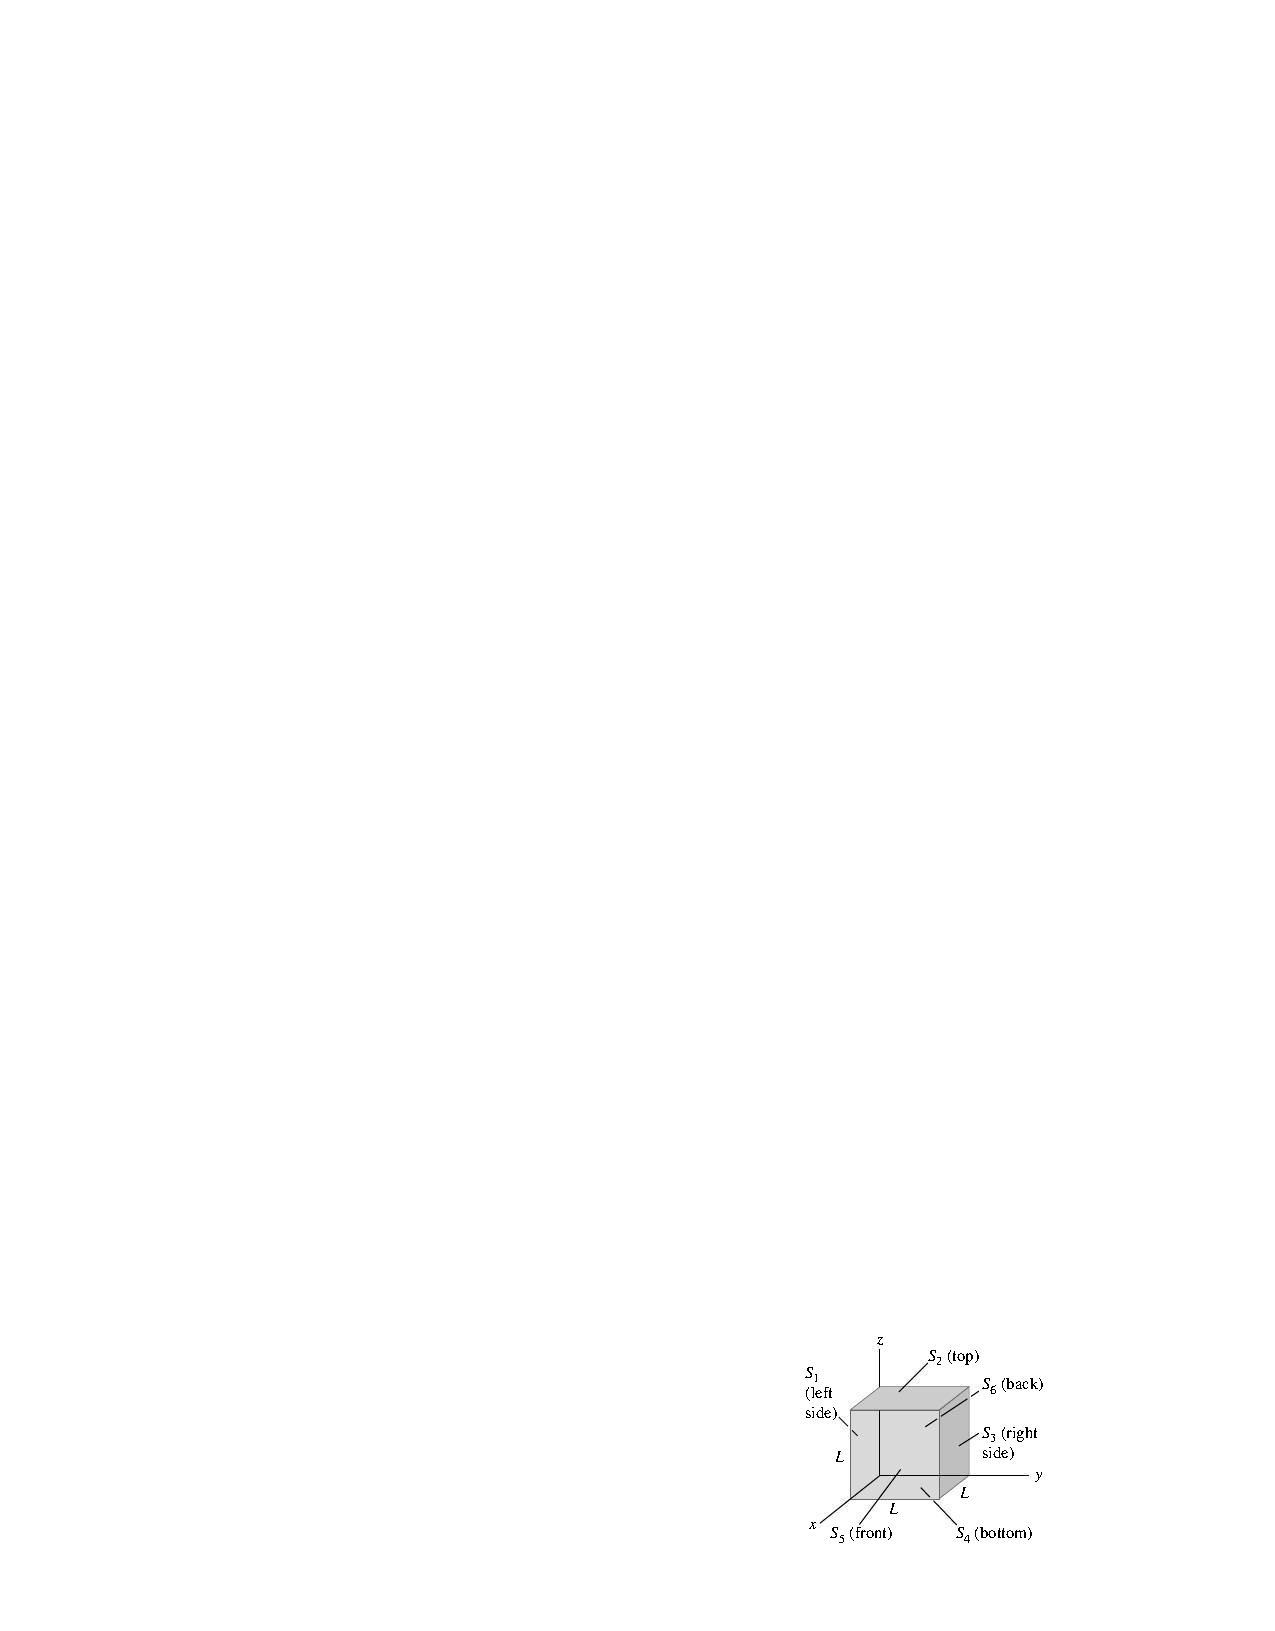
\includegraphics[width=\textwidth]{E22-6}
\center \textbf{Figure E22.6}
\end{minipage}

\newcommand{\PhiE}{\Phi_E}
\newcommand{\Qenc}{Q_\text{enc}}
\newcommand{\vA}{\vec{A}}
\newcommand{\jh}{\vec{\hat{j}}}
\newcommand{\kh}{\vec{\hat{k}}}

\begin{solution}
	\begin{enumerate}
		\item This is a problem about flux, so it's a problem about Gauss's law:
		\beq
			\PhiE = \oint \vE \cdot \dd{\vA} = \frac{\Qenc}{\ent}.
		\eeq
		For this first part, we'll be using the first equality with
		\beq
			\oint \vE \cdot \dd{\vA} = \vE \cdot \vA.
		\eeq
		For each face of the cube, we define the magnitude of the vector $\vA$ by the area of its face.  We define the direction by the unit normal~(perpendicular) to the face, pointing outward.  Looking at the picture, this gives us
		\begin{align*}
			\vA_1 &= - L^2 \,\jh, &
			\vA_2 &= L^2 \,\kh, &
			\vA_3 &= L^2 \,\jh, &
			\vA_4 &= -L^2 \,\kh, &
			\vA_5 &= L^2 \,\ih, &
			\vA_6 &= -L^2 \,\ih.
		\end{align*}
		Now we can find the flux through each of the faces:
		\begin{align*}
			\Phi_1 &= \vE \cdot \vA_1 = {\color{blue} 0}, &
			\Phi_3 &= \vE \cdot \vA_3 = {\color{blue} 0}, &
			\Phi_4 &= \vE \cdot \vA_4 = {\color{blue} 0}, &
			\Phi_6 &= \vE \cdot \vA_6 = {\color{blue} 0},
		\end{align*}
		and
		\begin{align*}
			\Phi_2 &= \vE \cdot \vA_2
			= \Ex L^3
			= (\SI{3.00}{\newton\per\coulomb\per\meter}) (\SI{3.00e-1}{\meter})^3 = 3^4 \times \SI{e-3}{\newton\square\meter\per\coulomb} \\
			&= {\color{blue} \SI{81.0e-3}{\newton\square\meter\per\coulomb}}, \\[1em]
			\Phi_5 &= \vE \cdot \vA_5
			= E_z L^3
			= (\SI{-5.00}{\newton\per\coulomb\per\meter}) (\SI{3.00e-1}{\meter})^3 = (5) 3^3 \times \SI{e-3}{\newton\square\meter\per\coulomb} \\
			&= {\color{blue} \SI{-135.0e-3}{\newton\square\meter\per\coulomb}}.
		\end{align*}
		
		\item Now we'll use the second equality of Gauss's law to find the charge.  The total flux is simply the sum of the (nonzero) results from (a):
		\beq
			\PhiE = \Phi_2 + \Phi_5 = \SI{-54.0e-3}{\newton\square\meter\per\coulomb}.
		\eeq
		Then
		\begin{align*}
			\Qenc &= \ent \PhiE
			= (\SI{8.86e-12}{\square\coulomb\per\newton\per\square\meter}) (\SI{-5.400e-2}{\newton\square\meter\per\coulomb})
			= (8.86) (5.4) \times \SI{e-14}{\coulomb} \\
			&= {\color{blue} \SI{-4.78e-13}{\coulomb}}.
		\end{align*}
	\end{enumerate}
\end{solution}

%\bigskip
\clearpage

\newcommand{\ra}{r_a}
\newcommand{\rb}{r_b}
\newcommand{\rh}{\vec{\hat{r}}}

\paragraph{Problem 24.11}
%\paragraph{Problem 4}
\begin{problem}
	A spherical capacitor contains a charge of \SI{3.30}{\nano\coulomb} when connected to a potential difference of \SI{220}{\volt}.  If its plates are separated by vacuum and the inner radius of the outer shell is \SI{4.00}{\centi\meter}, calculate
	
	\begin{enumerate}
		\item the capacitance,
		\item the radius of the inner sphere, and
		\item the electric field just outside the surface of the inner sphere.
	\end{enumerate}
\end{problem}

\begin{solution}
	\begin{enumerate}
		\item We just need to use the definition of capacitance:
		\beq
			C = \frac{Q}{V}
			= \frac{\SI{3.30e-9}{\coulomb}}{\SI{2.20e2}{\volt}}
			= \frac{3.3}{2.2} \times \SI{e-11}{\farad}
			= {\color{blue} \SI{1.50e-11}{\farad}}.
		\eeq
		
		\item We can relate the capacitor's capacitance to its geometry using the equation for a spherical capacitor, which is derived in Ex.~24.3.  The expression is
		\beq
			C = 4\pi\ent \frac{\ra \rb}{\rb - \ra},
		\eeq
		where $\ra$ is the inner radius and $\rb$ is the outer radius.  First we need to solve for the inner radius:
		\beq
			4\pi\ent = C \frac{\rb - \ra}{\ra\rb} = \frac{C}{\ra} - \frac{C}{\rb}
			\implies \frac{C}{\ra} = \frac{C}{\rb} + 4\pi\ent
			\implies \ra = \frac{C \rb}{C + 4\pi\ent \rb}.
		\eeq
		Plugging in the given $\rb$ and our result from (a) gives us
		\begin{align*}
			\ra &= \frac{(\SI{1.50e-11}{\farad}) (\SI{4.00e-2}{\meter})}{(\SI{1.50e-11}{\farad}) + 4\pi (\SI{8.86e-12}{\square\coulomb\per\newton\per\square\meter}) (\SI{4.00e-2}{\meter})} \\
			&= \frac{(1.5)(4) \times \num{e-13}}{[1500 + 4 (3.142) (8.86) (4)] \times \num{e-14}} \si{\meter}
			= \frac{6}{1945} \times \SI{e1}{\meter}
			= {\color{blue} \SI{3.08}{\cm}}.
		\end{align*}
		
		\item We can use Gauss's law.  If we enclose the inner sphere in a spherical Gaussian surface, our $\Qenc = \SI{3.30}{\nano\coulomb}$.  We know that the electric field will be the same as for a point charge located at the sphere's center.  Just outside the surface of the inner sphere, we are a distance $\ra$ away from the center.  Then
		\begin{align*}
			\vE &= \fk \frac{\Qenc}{\ra^2} \rh
			= (\SI{8.99e9}{\newton\square\meter\per\square\coulomb}) \frac{\SI{3.00e-9}{\coulomb}}{(\SI{3.08e-2}{\meter})^2} \rh
			= \frac{(8.99)(3)}{3.08} \times \SI{e4}{\newton\per\coulomb} \, \rh \\
			&= {\color{blue} (\SI{3.12e4}{\newton\per\coulomb}) \,\rh}.
		\end{align*}
	\end{enumerate}
\end{solution}

\end{document}